%!TEX root = ../Bachelorarbeit.tex
\chapter{Motivation}
\label{chap:Einleitung}
Die School of Design Thinking (D-School) lehrt die kreative Herangehensweise an Probleme und die Entwicklung einfallsreicher Lösungen. Die Lehre findet dabei in verschiedenen Kursen statt. Studierende können sich die Grundlagen im \gls{Basic-Track} aneignen und nach erfolgreicher Teilnahme ihr Wissen im  \gls{Advanced-Track} vertiefen. Neben den studentischen Kursen bietet die D-School auch Weiterbildungskurse für Unternehmen an.

In der Regel besteht ein D-School Kurs aus mehreren multidisziplinaren Kleingruppen von üblicherweise sechs Teilnehmern, die gemeinsam an einem Projekt arbeiten. Das Projektthema wird dabei entweder von der D-School selbst oder, vor allem bei längeren Projekten, von externen Projektpartnern vorgeschlagen. 

Bei der Arbeit an den Projekten durchlaufen die Teilnehmenden verschiedene Phasen: Während dabei zunächst das Verstehen und Beobachten des Problemfeldes im Vordergrund stehen, wird anschließend ein Standpunkt definiert. Es folgt die Phase der Ideenfindung, an die die Erstellung eines Prototypen anknüpft. Dieser Prototyp wird zum Schluss mit geeigneten Versuchspersonen getestet. Die verschiedenen Phasen sind in der Abbildung \ref{fig:dschool-prozess} dargestellt. Im Verlauf der Phasen entstehen unterschiedlichste Dokumente, welche die Lösungsfindung dokumentieren. (vgl. \cite{design-thinking})

\begin{figure}[h]  
  \centering     
  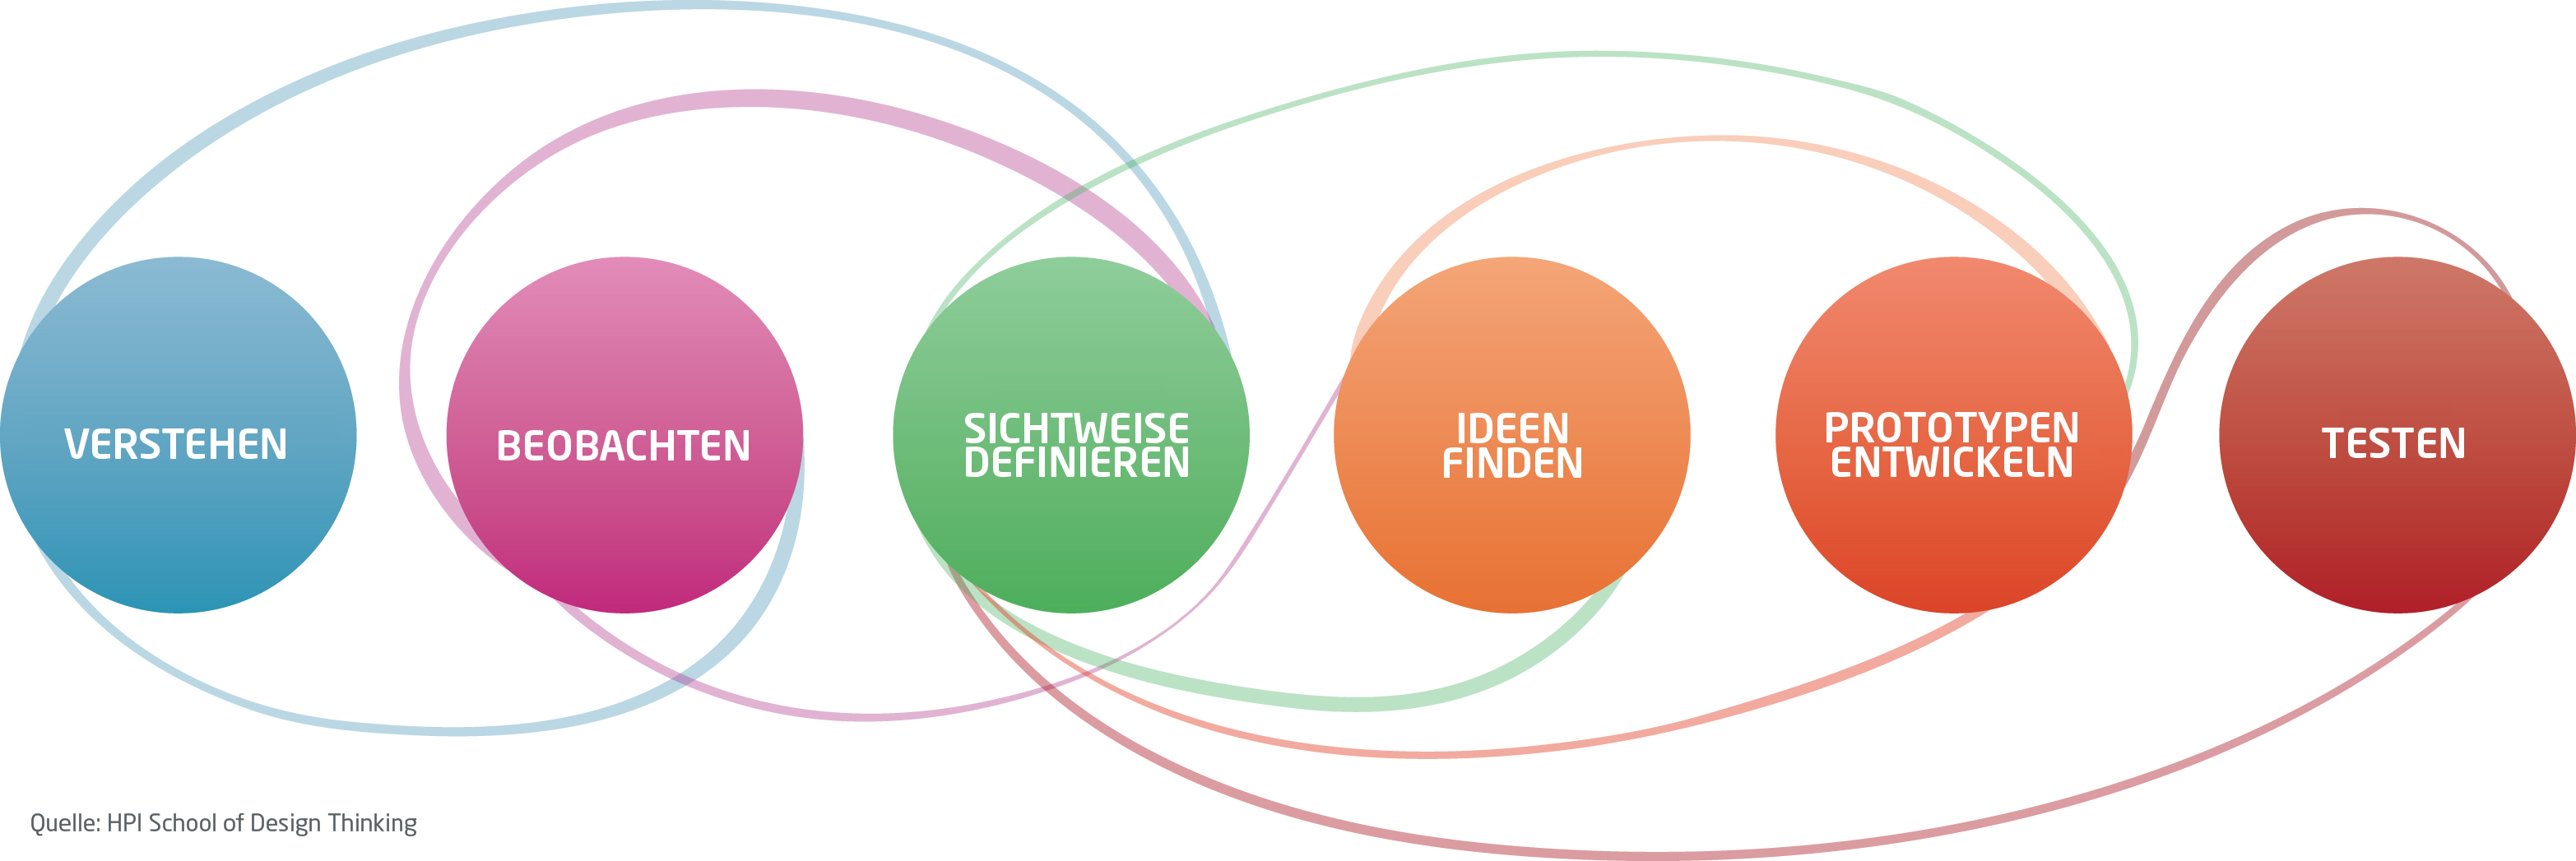
\includegraphics[width=1.0\textwidth]{img/dschool_prozess.jpg}  
   \caption{Phasen des D-School-Prozesses\protect\footnotemark}
  \label{fig:dschool-prozess} 
\end{figure}
\footnotetext{Quelle: \url{http://www.hpi.uni-potsdam.de/fileadmin/hpi/presse/pressedownloads/allgemeine_fotos/HPI_School_of_Design_Thinking_-_Prozess_dt.jpg}}

Im Verlauf des Projektes kommt es durchaus vor, dass ein Team eine Phase mehrmals durchläuft oder in eine vorherige Phase zurückkehrt. Dies erschwert die Organisation der Dokumente, z.B. in einer einfachen hierarchischen Struktur. Weiterhin ist es schwierig allein aus den Dokumenten deren Entstehungsreihenfolge und Bedeutung zu erfassen. Meist entstehen während eines drei Monate andauernden Projektes verschiedenste Präsentationen, Zusammenfassungen, Prototypen, Bilder von Whiteboards und Interviewdokumentationen. Diese werden in der Regel in der von den Studierenden bevorzugten Art und Weise gespeichert und verwaltet, beispielsweise mit Hilfe von Dropbox\footnote{\url{http://www.dropbox.com}}, Google Docs\footnote{\url{http://drive.google.com}} oder \gls{Box}\footnote{\url{http://box.com}}.

Das Verständnis der Dokumentation ist sowohl für das Projekt selbst, zum Verstehen und Erlernen des Prozesses, als auch als Ideenquelle für zukünftige Projekte wichtig. Ferner sind die erstellten Artefakte nützlich um neue Projektpartner zum werben, welche die Projekte anbieten. 

\section{Systemanforderungen}
Im Verlauf des Projektes wurden in Zusammenarbeit mit Studierenden und den Mitarbeitern der D-School verschiedene Anforderungen an Project-Zoom als Projektverwaltungs- und Dokumentationstool aufgestellt (vgl. \cite{requirements}).  Aus diesen leiten sich später die umgesetzte Architektur und die verwendeten Technologien ab. Hier aufgeführt sind nur die für diesen Teil des Projektes wichtigsten und relevanten Anforderungen. Für eine Analyse der Nutzergruppen und deren Bedürfnissen sei auf \cite{requirements}  verwiesen.

\paragraph{Funktionale Anforderungen}
\label{sec:functional}
\begin{labeling}{\textbf{NF1:}}
  \item[\textbf{F1:}] Es muss sichergestellt werden, dass kein unautorisierter Nutzer auf Daten Zugriff hat, die geschützt sind.

  Dies ergibt sich aus dem Vorhandensein von Geheimhaltungsverträgen der Projekte und dem Wunsch der D-School den Zugriff zu beschränken. 

  \item[\textbf{F2:}] Innerhalb der Anwendung soll die Daten aus Filemaker, Box, Netzwerkdateisysteme und Facebook aggregiert werden.

  Die Angegebene Reihenfolge entspricht dem Wunsch der Umsetzung von der D-School.

  \item[\textbf{F3:}] Aggregierte Daten sollen nicht gelöscht werden. 

  Es kann durchaus vorkommen, dass Daten in aggregierten Quellen nach einiger Zeit gelöscht werden müssen. Die Anwendung soll die Daten dann weiterhin vorhalten können. Dass eine Ressource in der originalen Quelle nicht mehr vorhanden ist, kann zum Beispiel durch eine Markierung in einer Datenbank erfolgen.

  \item[\textbf{F4:}] Die Anwendung von neuen Datenquellen muss möglich sein. Das Core-Backend soll dabei unverändert bleiben.

  Über die Zeit verändern sich die von den Studierenden verwendeten Werkzeuge zur Dokumentation. 

  \item[\textbf{F5:}] Es dürfen keine Aggregierten Daten in deren Quellen verändert werden.

  Die Anwendung soll auf externe Daten nur lesend zugreifen. Dies dient dem Schutz der Datenquellen.

  \item[\textbf{F6:}] Die Studierenden sollen in der Lage sein, die Anwendung außerhalb der D-School verwenden zu können. 

  Dies ist wichtig, da die Studierenden meist nur zwei Tage in der Woche in der D-School verbringen. Zum Teil treffen sich die Projekt-Teilnehmer außerhalb der D-School mit Interviewpartnern und Projektpartnern, welche am Stand des Projektes interessiert sind. 
\end{labeling}

\paragraph{Nichtfunktionale Anforderungen}
\label{sec:nonfunctional}

\begin{labeling}{\textbf{NF1:}}
  \item[\textbf{NF1:}] Es sollen 100 Nutzer gleichzeitig in der Lage sein, das Backend zu Nutzen.

  Dies entsteht aus der Abschätzung für die Anzahl aller Teilnehmer und Teacher von etwa 100 Nutzern. Da keine anderen Nutzer Zugriff auf das System haben sollen, entspricht dies einer oberen Schranke für die Anzahl der gleichzeitigen Nutzer. 

  \item[\textbf{NF2:}]  Der Server muss die Updates aus den Datenquellen innerhalb von einer Minute verarbeiten.

  Umso schneller die Updates vom System verarbeitet werden, desto eher können die Nutzer mit den Daten in der Anwendung arbeiten. Die Grenze von einer Minute wurde gewählt, da dies einerseits eine realistische Zeitspanne für notwendige Berechnungen ist und andererseits das Arbeiten mit dem System durch den Studierenden ermöglicht.
\end{labeling}


\section{Idee von Project-Zoom}
 
Im Entwicklungsprozess einer Lösung zur Verbesserung der Dokumentation in der D-School wurde auf den D-School-Prozess zurückgegriffen. Dies ermöglichte einen sehr guten Einblick in die Arbeitsweise der Teilnehmer in den Projekten der D-School. 

\begin{figure}[h]  
  \centering     
  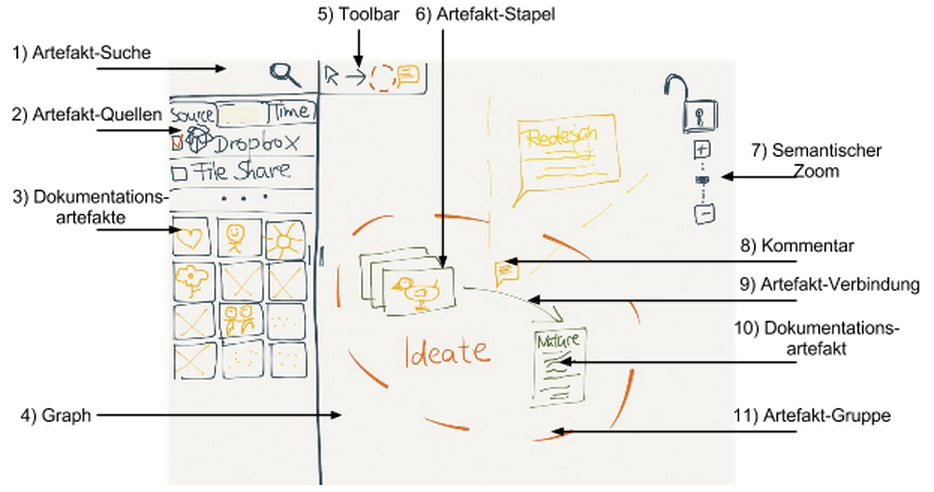
\includegraphics[width=1.0\textwidth]{img/projectzoom_prototype.png}  
   \caption{Prototyp einer Übersicht über den Dokumentationsprozess eines Projektes}
  \label{fig:projectzoom_prototype} 
\end{figure}

In mehreren Iterationen wurde so Project-Zoom entwickelt und verfeinert. Einer der ersten Entwürfe der Nutzoberfläche ist in Abbildung \ref{fig:projectzoom_prototype} zu sehen. Das Konzept von Project-Zoom ist die Verbindung einer Projektübersicht mit einem Projekteinblick. Der Nutzer soll also in der Lage sein, einen Überblick über alle Projekte und bei Bedarf einen tieferen Einblick in das Projekt bekommen zu können.

Project-Zoom soll der Verbesserung der Dokumentation dienen. Dazu sollen die von den Studierenden erzeugten Artefakte durch manuelles Anordnen in eine Form gebracht werden, welche den Prozess der Gruppe visualisiert. Die Mitarbeiter der D-School können diese entstandenen Graphen anschließend nutzen um die Projektverläufe zu analysieren und gegebenenfalls den D-School Prozess anpassen (vgl. Interview mit Claudia Nikolai im Anhang \ref{sec:interview_nikolai}).

Für eine reibungslose Integration des Systems ist vor allem die Anbindung an bereits existierende IT-Systeme  und die von den Studierenden für das Projekt verwendete Software wichtig (vgl. REQXXX). Änderungen an diesen externen Diensten und der Auswahl der anzubindenden Datenspeicher ist über die Zeit sehr wahrscheinlich. Deshalb muss das System modular aufgebaut sein, um nachträglich neue Dienste Anbinden zu können ohne den Backend-Core zu verändern.

\section{Abgrenzung}
Die Arbeit beschreibt und bezieht sich auf das Bachelorprojekt „From Creative Ideas to Well-Founded Engineering“ und das umgesetzte Softwaresystem Project-Zoom. Insgesamt haben sechs Studierende an dem Projekt gearbeitet, die in ihren Bachelorarbeiten aus verschiedenen Blickwinkeln und mit verschiedenen Schwerpunkten Project-Zoom beschreiben.

Tom Herolds Arbeit \cite{bp-tomh} beinhaltet die Interaktion mit kontextsensitiven Graphen. Dabei geht es darum, den Umgang der Studierenden mit der Nutzeroberfläche so intuitiv wie möglich zu gestallten und den Nutzer bei der Erfassung dokumentationsrelevanter Eigenschaften zu unterstützen.

Die Ausführungen von Anita Diekhoff \cite{bp-anita}  beschäftigen sich mit der ...

Norman Rzepkas Bachelorarbeit \cite{bp-norman} thematisiert die webbasierte, eventgesteuerte, clientseitige Architektur von Project-Zoom. Hier wird näher darauf eingegangen, wie die Daten von der Datenbank, über das Backend asynchron an den Client ausgeliefert werden.

Die Bachelorarbeit von Dominic Bräunlein \cite{bp-dome} erläutert das Generieren und Bereitstellen von semantischen \gls{Thumbnails}, um dem Nutzer das Erkennen der Dokumente seines Projektes zu erleichtern und somit selbst bei wenig verfügbarem Platz so viele Informationen eines Dokumentes anzeigen zu können wie möglich. 

Thomas Werkmeister befasst sich in seiner Arbeit \cite{bp-tewe} mit der Anbindung externer Systeme zur Integration von Daten. Diese aggregierte Datenbasis ist die Grundlage für die Wissensbasis und die einzelnen Projekte.

\begin{figure}[h]  
  \centering     
  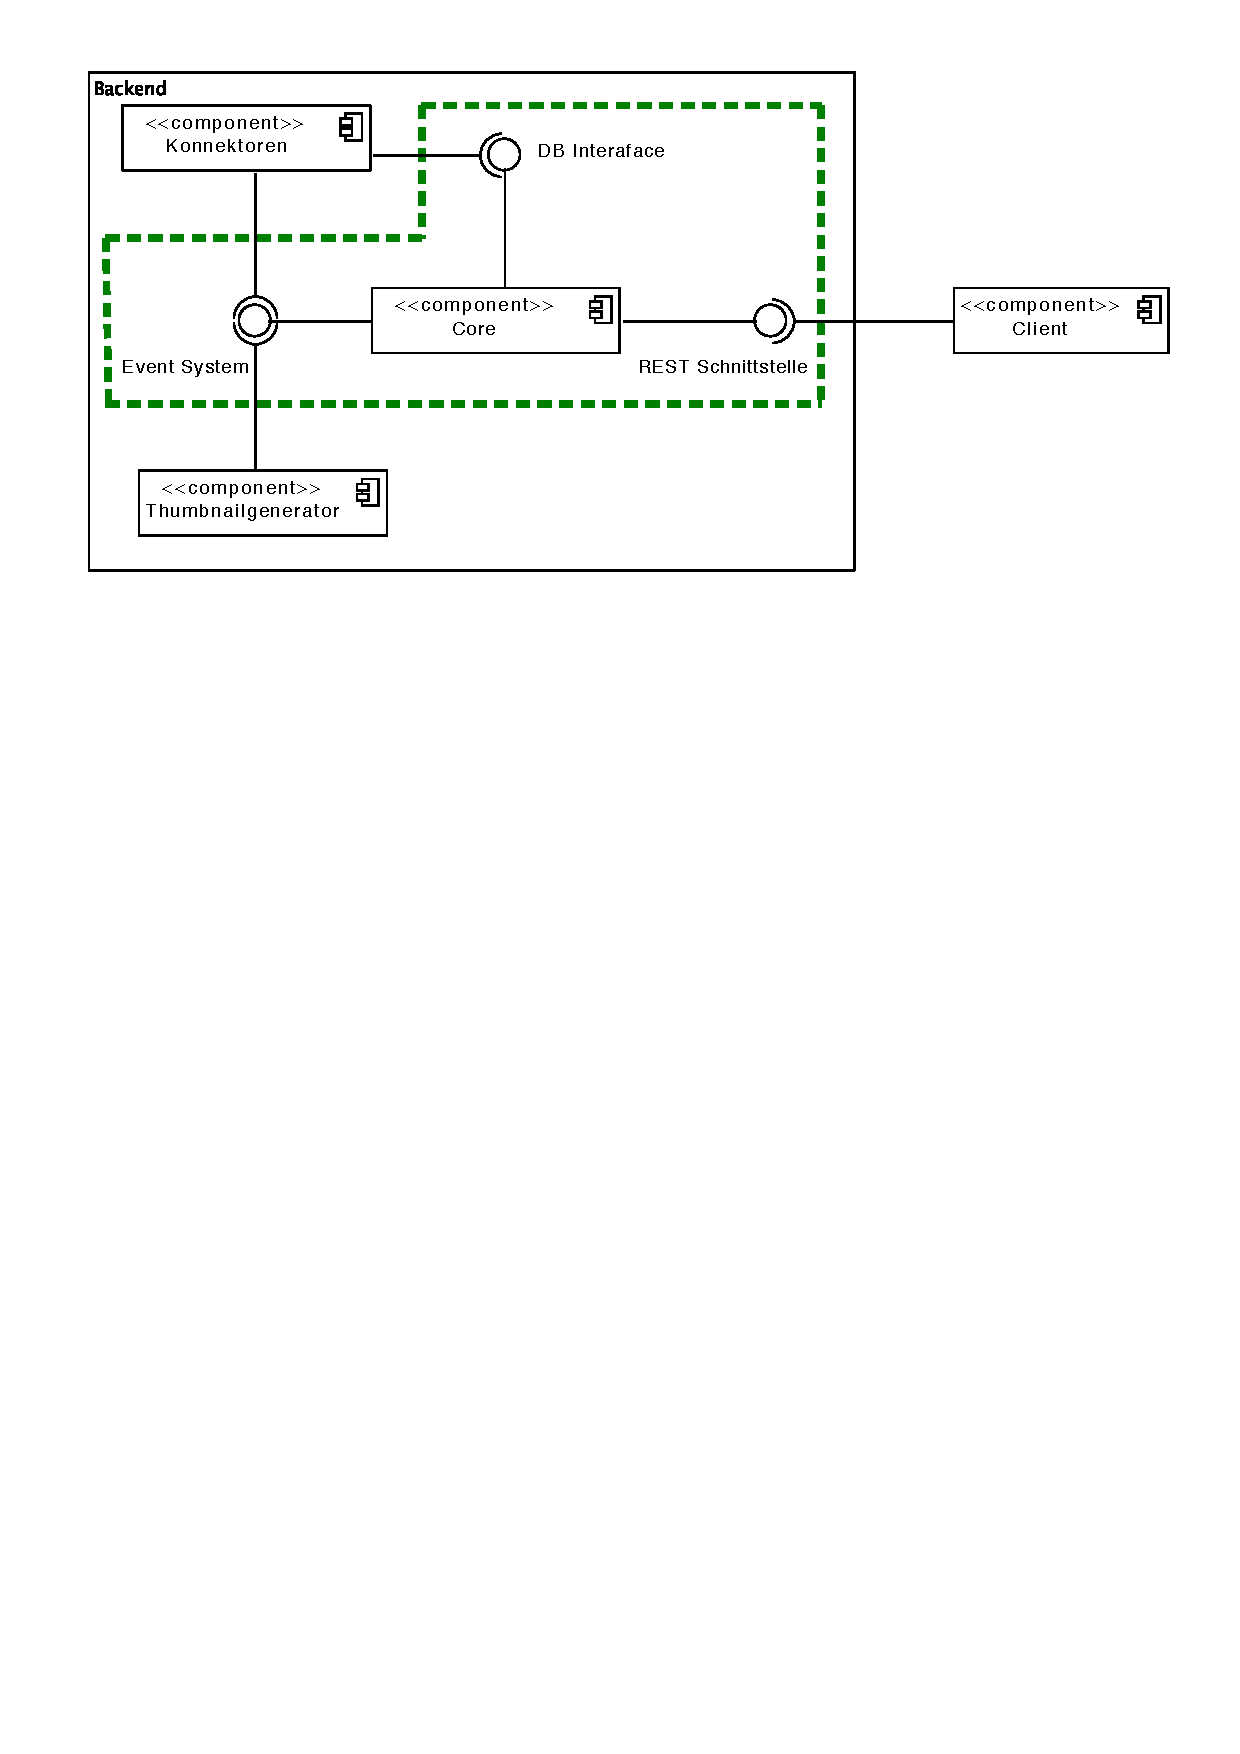
\includegraphics[width=1.0\textwidth]{img/architecture_overview.pdf}  
   \caption{Überblick über die verschiedenen Packete und ihre Schnittstellen; In gestricheltem Rahmen der für diese Arbeit relevante Teil der Architektur}
  \label{fig:architecture-overview} 
\end{figure}

Die Abbildung \ref{fig:architecture-overview} zeigt einen groben Überblick über die Architektur des Systems. Der für diese Arbeit relevante Teil ist dabei gestrichelt eingerahmt. Die Komponenten, die in den Arbeiten \cite{bp-tewe} (Konnektoren) und \cite{bp-dome} (Thumbnailgenerator) beschrieben sind, sind mit dem hier erläuterten Systemteil mittels eines Eventsystems verbunden. Das Client-Frontend ist über eine REST-Anbindung\footnote{vgl. Konzept des Representational State Transfer in \cite{rest}} an das Server-Backend angeschlossen. Mit der clientseitigen Implementierung der REST-Schnittstelle beschäftigt sich \cite{bp-norman}.

In dieser Arbeit wird zunächst ein Überblick über das Gesamtsystem gegeben. Dazu werden die Anforderungen der D-School an das Backend analysiert, welche als Grundlage für die Wahl der verwendeten Technologien dienen. Anschließend wird die Architektur des Backends näher erläutert. Hier liegt der Hauptfokus zunächst auf einer neuen Art und Weise, eine Datenbank an eine Webapplikation anzubinden. Im Anschluss werden einige Feinheiten und ausgewählte Stellen der Datenmodellierung von Project-Zoom beleuchtet. Den Abschluss bildet die architekturelle Grundlage zur Anbindung externer Systeme für die Erweiterung von Project-Zoom.

%\zitat{"`Ein Zitat kann manchmal helfen ;-)"' (\cite{TODO})} 